% !TeX root = tesis.tex

En esta sección introducimos las curvas elípticas sobre un cuerpo, y las dotamos de una estructura de grupo abeliano. Las curvas elípticas presentan propiedades de seguridad criptográfica favorables, en particular, para niveles de seguridad comparables, los grupos de curvas elípticas permiten tamaños de parámetros significativamente menores que los grupos multiplicativos clásicos.

\begin{definition}[Curva elíptica]
	Sea $\K$ un cuerpo con $\charac{\K} \neq 2,3$. Una curva elíptica $\E$ sobre $\K$ es una curva, junto con un punto distinguido $\OO$, que puede describirse mediante una ecuación de la forma
	$$\E: y^2 = x^3 + ax + b, \quad a,b \in \K,$$
	y sujeta a la condición de no singularidad $4a^3 + 27b^2 \neq 0$.
	
	El conjunto de puntos de la curva elíptica sobre $K$ se define como
	$$\E(\K) = \{(x,y) \in \K \times \K: y^2 = x^3 + ax + b\} \cup \{\OO\},$$
	donde $\OO$ denota el punto del infinito o punto identidad.
\end{definition}

La condición de no singularidad garantiza que la curva no posee puntos singulares, y por lo tanto que la curva es lisa. Es decir, si consideramos la función en dos variables $F(x,y) = y^2 - x^3 - ax - b$, sus derivadas parciales son $\frac{\partial F}{\partial x}(x,y) = -3x^2 - a$, y $\frac{\partial F}{\partial y}(x,y) = 2y$. Un punto de la curva es singular si ambas derivadas parciales de $F$ se anulan en él.

\begin{definition}[Definición geométrica de suma en curvas elípticas]
	Sea $\K$ un cuerpo, y $\E(\K)$ una curva elíptica. Dados $P, Q \in \E(\K)$, se define la suma $+: \E(\K) \times \E(\K) \to \E(\K)$ desde una perspectiva geométrica, como:
	\begin{enumerate}
		\item Se considera la recta que pasa por $P$ y $Q$. En el caso particular $P = Q$, se toma la recta tangente a la curva en $P$. En el caso particular $Q = -P$, la recta es vertical.
		\item La recta interseca a la curva elíptica en un tercer punto $R$ (contando multiplicidades).
		\item Si $R'$ es la reflexión de $R$ por el eje $x$, se define $P + Q := R'$. En el caso particular de la recta vertical, tenemos $Q = -P$ y se define $P + Q := \OO$.
	\end{enumerate}
\end{definition}

\begin{figure}[ht]
	\centering
	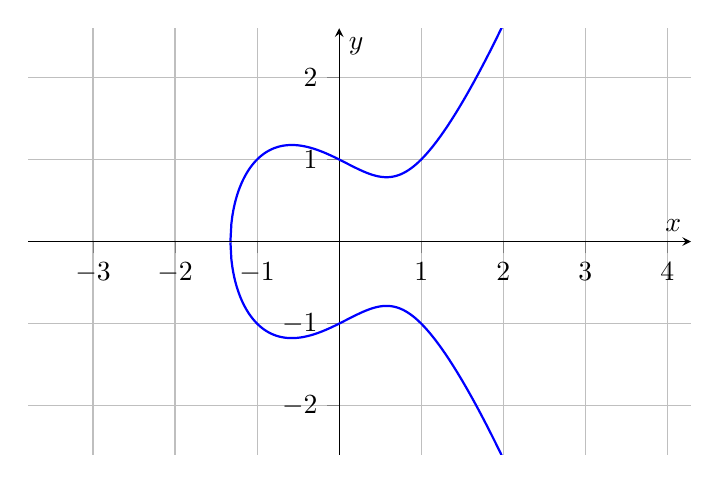
\begin{tikzpicture}
		\begin{axis}[
			axis lines = middle,
			axis equal,
			xlabel = $x$,
			ylabel = $y$,
			xmin = -1.6,
			xmax = 2.1,
			ymin = -2.6,
			ymax = 2.6,
			samples = 300,
			domain = -1.3247:2,
			width = 10cm,
			height = 7cm,
			grid = both,
			tick align = outside
			]
			
			% Rama superior
			\addplot[blue, thick] {sqrt(x^3 - x + 1)};
			
			% Rama inferior
			\addplot[blue, thick] {-sqrt(x^3 - x + 1)};
		\end{axis}
	\end{tikzpicture}
	\caption{Curva elíptica en $\poly{\R}$ asociada a la ecuación $\E: y^2 = x^3 - x + 1$.}
	\label{fig:curva-eliptica-real}
\end{figure}


La introducción del punto $\OO$ es necesaria para que la suma de puntos esté definida en todos los casos, en particular cuando se suman puntos opuestos cuya recta secante es vertical. Sin este punto adicional, la operación no sería cerrada en $\E(\K)$. Esta operación cumple el resto de propiedades para poder considerar a $(\E(\K), +)$ como un grupo abeliano:
\begin{itemize}
	\item $P + \OO = \OO + P = P$ para todo $P \in \E(\K)$ (elemento neutro).
	\item $P + (-P) = \OO$ para todo $P \in \E(\K)$ (elemento inverso). Un detalle geométrico relevante es que $-P$ se obtiene al reflejar $P$ por el eje $x$.
	\item $P + (Q + R) = (P + Q) + R$ para todos $P, Q, R \in \E(\K)$ (asociatividad).
	\item $P + Q = Q + P$ para todos $P, Q \in \E(\K)$ (conmutatividad).
\end{itemize}

Por convención, utilizaremos notación aditiva en vez de multiplicativa al trabajar con grupos de curva elíptica. Dados $n \in \N$ y $P \in \E(\K)$, podemos definir $nP := P + P + \ldots + P$, donde hay $n$ sumandos.

Al pasar a considerar curvas elípticas sobre cuerpos finitos (i.e., los que nos serán útiles criptográficamente), es decir de la forma $\E(\Fp)$ con $p > 3$, la interpretación geométrica deja de ser literal, aunque resulta útil como guía conceptual. Pero seguimos teniendo un grupo abeliano, y en particular la operación de suma sigue siendo cerrada. Sin embargo, no tiene sentido definir la operación de forma geométrica, sino que deberemos hacerlo algebraicamente. Observar durante la definición cómo nos apoyamos en las definiciones geométricas para hacer las definiciones algebraicas.

\begin{figure}[ht]
	\centering
	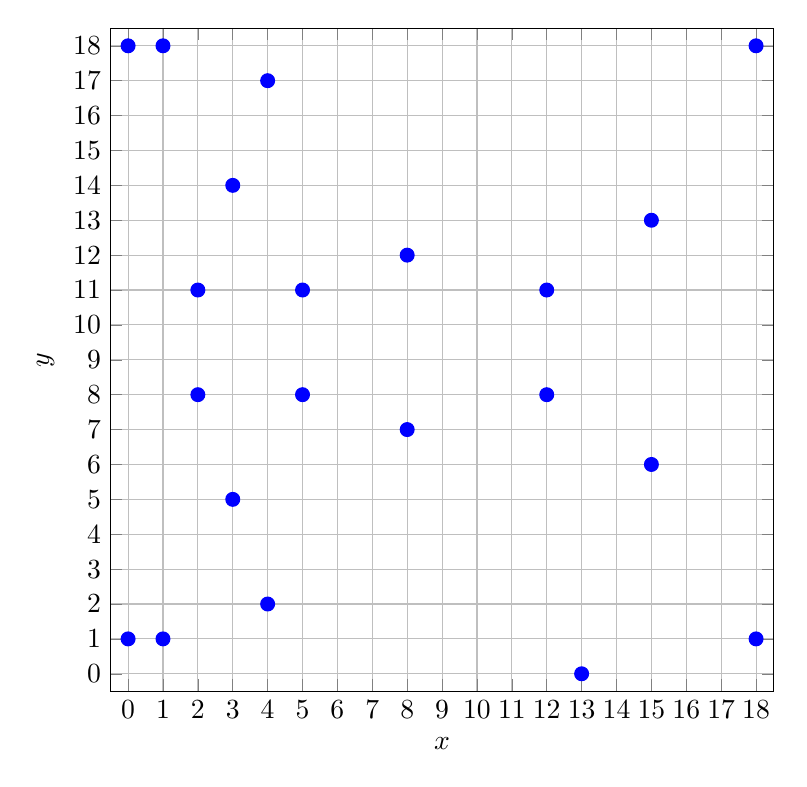
\begin{tikzpicture}
		\begin{axis}[
			axis equal,
			xmin = -0.5,
			xmax = 18.5,
			ymin = -0.5,
			ymax = 18.5,
			xtick = {0,...,18},
			ytick = {0,...,18},
			grid = both,
			xlabel = $x$,
			ylabel = $y$,
			width = 10cm,
			height = 10cm
			]
			\addplot[
			only marks,
			mark = *,
			mark size = 2.5pt,
			blue
			]
			coordinates {
				(0,1) (0,18)
				(1,1) (1,18)
				(2,8) (2,11)
				(3,5) (3,14)
				(4,2) (4,17)
				(5,8) (5,11)
				(8,7) (8,12)
				(12,8) (12,11)
				(13,0)
				(15,6) (15,13)
				(18,1) (18,18)
			};		
		\end{axis}
	\end{tikzpicture}
	\caption{Curva elíptica en $\F_{19}[x]$ asociada a la ecuación $\E: y^2 = x^3 - x + 1$.}
	\label{fig:curva-eliptica-f19}
\end{figure}

\begin{definition}[Definición algebraica de suma en curvas elípticas]
	Sea $\K$ un cuerpo finito, sea $\E(\K)$ una curva elíptica y sean $P, Q \in \E(\K)$. Se define la suma $+: \E(\K) \times \E(\K) \to \E(\K)$ desde una perspectiva algebraica mediante fórmulas explícitas y el siguiente algoritmo:
	\begin{enumerate}
		\item Si $P = \OO$, entonces $P + Q := Q$. Similarmente, si $Q = \OO$, entonces $P + Q := P$.
		\item Si $P, Q \neq \OO$, entonces son puntos de la forma $P = (x_P, y_P)$, $Q = (x_Q, y_Q)$ con coordenadas en $\Fp$. Si $Q = -P$, lo que es equivalente a $x_P = x_Q$ y $y_P = -y_Q$, entonces $P + Q := \OO$.
		\item Se calcula la pendiente $\lambda$ de la recta que pasa por $P$ y $Q$.
		\begin{itemize}
			\item En el caso $P = Q$, es una recta tangente a $P$ y $\lambda := \frac{3x_P^2 + a}{2y_P}$.
			\item En el caso $P \neq Q$, se calcula de forma usual: $\lambda := \frac{y_Q - y_P}{x_Q - x_P}$.
		\end{itemize}
		\item Para $x^* := \lambda^2 - x_P - x_Q$ y $y^* = \lambda(x_P - x^*) - y_P$, se define $P + Q := (x^*, y^*)$.
	\end{enumerate}
\end{definition}

Una curva elíptica sobre cuerpos finitos tiene finitos puntos. Pero es notable que, en general, $|\E(\Fq)| \neq |\Fq| = q$. La cota de Hasse establece un límite preciso para el número de puntos racionales de una curva elíptica definida sobre un cuerpo finito.

\begin{theorem}[Cota de Hasse]
	Sea $\Fq$ un cuerpo finito, y sea $\E(\Fq)$ una curva elíptica. Entonces, $|\E(\Fq)| - (q + 1)| \leq 2\sqrt{q}$.
\end{theorem}

En particular, es relevante en numerosos protocolos criptográficos que $|\E(\Fq)|$ tenga un divisor primo grande. Usualmente se eligen curvas elípticas donde $|\E(\Fq)| = hr$, donde $r$ es un primo grande y $h$ (llamado el \textit{cofactor} de la curva) es un número pequeño, como 1, 2, o 4. Ahora sí estamos preparados para adentrarnos en los subgrupos cíclicos de una curva elíptica sobre un cuerpo finito.

\begin{definition}[Orden de un punto en una curva elíptica]
		Sea $\Fq$ un cuerpo finito, y sea $\E(\Fq)$ una curva elíptica. Para cada punto $P \in \E(\Fq)$, definimos su orden como el menor $r \in \N$ tal que $rP = \OO$. Es decir, $|\gen{P}|$ para $\gen{P} \subset \E(\Fq)$.
\end{definition}

Observamos que el orden de $P$ siempre existe y es un divisor del orden de $\E(\Fq)$ por el corolario del Teorema de Lagrange. Dentro de este grupo cíclico podemos volver a considerar el \DLP, pero sobre un grupo de curva elíptica.

\begin{definition}[\ECDLP]
		Sea $\Fq$ un cuerpo finito, y sea $\E(\Fq)$ una curva elíptica. Dados un punto generador $G \in \E(\Fq)$ y un punto $P \in \gen{G}$, el problema del logaritmo discreto sobre curvas elípticas (\ECDLP) es encontrar un $k \in \N$ tal que $P = kG$.
\end{definition}

En este contexto, se entiende por qué es útil buscar que el orden $r$ de $\gen{G}$ sea un número primo grande. A diferencia del \DLP en el grupo multiplicativo $\Fmul{p}$, los algoritmos conocidos más eficientes para resolver el \ECDLP para cualquier curva elíptica son genéricos en la estructura de grupo, por lo que su complejidad está en $\BigOmega(\sqrt{r})$. Esta diferencia algorítmica se traduce en una ventaja práctica en términos de bits de seguridad para algoritmos criptográficos, y por lo tanto en operaciones más rápidas, menos uso de memoria, claves de menor tamaño, y pruebas más pequeñas. En este contexto, las claves privadas serán de la forma $k \in \Fr$, mientras que sus claves públicas derivadas serán de la forma $K = kG \in \E(\Fq)$.

\begin{table}[h]
	\centering
	\begin{tabular}{ccc}
		\toprule
		\textbf{Bits de seguridad} &
		\textbf{$\Fmul{p}$ (\DLP clásico)} &
		\textbf{$\E(\Fp)$ (\ECDLP)} \\
		\midrule
		128 & $\sim 3072$ bits & $\sim 256$ bits \\
		192 & $\sim 7680$ bits & $\sim 384$ bits \\
		256 & $\sim 15360$ bits & $\sim 512$ bits \\
		\bottomrule
	\end{tabular}
	\caption{Comparación de tamaños de parámetros para niveles de seguridad equivalentes.}
	\label{tab:security-comparison}
\end{table}

Sin embargo, existen curvas elípticas tales que existen algoritmos más eficientes (e incluso polinomiales) para resolver el \ECDLP. Esto hace que seleccionar qué curvas elípticas usar para los protocolos criptográficos no dependa solamente de la eficiencia de las operaciones, sino también de las características de la curva. Estas consideraciones motivan el estudio detallado de subgrupos cíclicos de orden primo, que constituyen el entorno algebraico fundamental para numerosas construcciones criptográficas modernas.

Si alguien descubre un algoritmo para resolver el \ECDLP en forma eficienta para alguna familia de curvas, se pasan a considerar al conjunto de curvas mal elegidas, y pasan a estar prohibidas para uso en criptografía. Decimos que un algoritmo de este tipo es un \textbf{ataque} criptográfico. El lector interesado puede referirse a ataques a curvas anómalas \cite{Smart1999}, al \textit{MOV attack} sobre curvas supersingulares \cite{Menezes1993}, o a los ataques con el algoritmo \textit{Weil Descent} \cite{Hess2005}.

Veremos que hay varias curvas elípticas que son usadas en distintas partes del proyecto. En general, a la hora de describir curvas elípticas sobre cuerpos finitos, vamos a diferenciar los siguientes parámetros:
\begin{itemize}
	\item El cuerpo base $\Fq$ sobre el que está construido la curva $\E(\Fq)$, para un primo $q \in \N$.
	\item Un generador $G \in \E(\Fq)$ de un subgrupo $\gen{G} \subset \E(\Fq)$.
	\item El cuerpo escalar $\Fr$, donde $r \in \N$ es el orden del subgrupo generado por $G$. Idealmente, $r$ será un primo grande.
\end{itemize}
